\documentclass[tikz,border=8pt]{standalone}
% Shared look for every TikZ diagram. Load with \input{../../tools/tikz-style.tex}
\usepackage[T1]{fontenc}
\usepackage{lmodern}
\renewcommand{\sfdefault}{lmr}  % diagrams use the same serif as the text
\usetikzlibrary{arrows.meta, positioning, shapes.geometric, calc, fit, backgrounds}
\definecolor{cblue}{HTML}{4C78A8}
\definecolor{corange}{HTML}{F58518}
\definecolor{cgreen}{HTML}{54A24B}
\definecolor{cred}{HTML}{E45756}
\definecolor{cpurple}{HTML}{B279A2}
\definecolor{cgrey}{HTML}{6B6B6B}
\tikzset{
  every picture/.style={font=\sffamily, line width=1.2pt},
  box/.style={draw=#1, fill=#1!12, rounded corners=4pt, align=center, inner sep=7pt, minimum height=1.1cm},
  box/.default=cgrey,
  arrow/.style={-{Stealth[length=3mm]}, draw=cgrey, line width=1.4pt},
  title/.style={font=\sffamily\bfseries\Large},
  note/.style={font=\sffamily\small, text=cgrey, align=center},
}
\AtBeginDocument{\hyphenpenalty=10000 \exhyphenpenalty=10000}

% Section 3 worked example: three samples of size 3, each mean marked, then the three means on one line.
\begin{document}
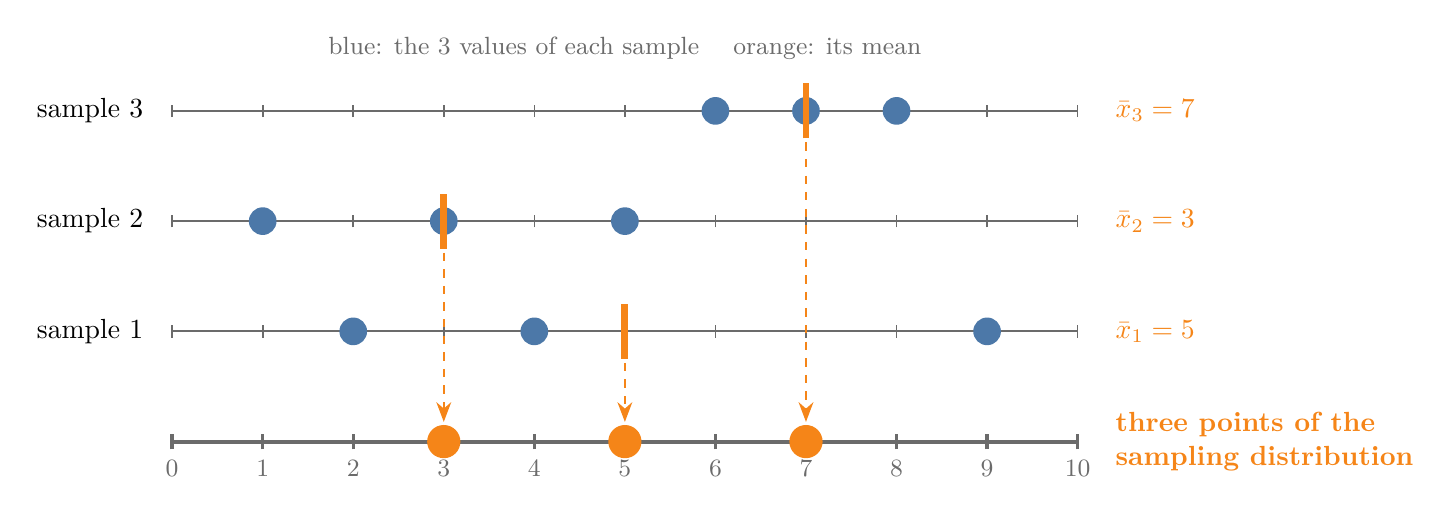
\begin{tikzpicture}[x=1.15cm]
  \foreach \row/\vals/\m/\y in {1/{2,4,9}/5/1.4, 2/{1,3,5}/3/2.8, 3/{6,7,8}/7/4.2} {
    \draw[cgrey, line width=0.8pt] (0,\y) -- (10,\y);
    \foreach \t in {0,...,10} \draw[cgrey, line width=0.6pt] (\t,\y-0.08) -- (\t,\y+0.08);
    \node[anchor=east, font=\sffamily] at (-0.2,\y) {sample \row};
    \foreach \v in \vals \fill[cblue] (\v,\y) circle (5pt);
    \draw[corange, line width=2.5pt] (\m,\y-0.35) -- (\m,\y+0.35);
    \node[anchor=west, font=\sffamily, text=corange] at (10.3,\y) {$\bar{x}_{\row} = \m$};
    \draw[corange, dashed, line width=0.9pt, -{Stealth[length=2.5mm]}] (\m,\y-0.4) -- (\m,0.25);
  }
  \draw[cgrey, line width=1.4pt] (0,0) -- (10,0);
  \foreach \t in {0,...,10} {\draw[cgrey] (\t,-0.1) -- (\t,0.1); \node[below, font=\sffamily\small, text=cgrey] at (\t,-0.1) {\t};}
  \foreach \m in {3,5,7} \fill[corange] (\m,0) circle (6pt);
  \node[anchor=west, font=\sffamily\bfseries, text=corange, align=left] at (10.3,0) {three points of the\\sampling distribution};
  \node[font=\sffamily\small, text=cgrey] at (5,5.0) {blue: the 3 values of each sample \quad orange: its mean};
\end{tikzpicture}
\end{document}
